\section{Results and discussion}
The number of fringes was plotted against the pressure change for the different gases and is found in Fig. \ref{fig:measurements}. As one can see in the figures, all gases showed a linear relation which was expected according to the theory. When comparing Fig. \ref{fig:Helium} with the others, the number of fringes is a lot lower. This means that the index of refraction must be considerably lower for helium. It also implies that the relative error in the result will probably be larger in this result in comparison to the others.

The linear fit parameters are found in Tab. \ref{tab:linearFits}. As expected, the slope $a$ for helium is a lot lower than the other slopes. From these slopes, the refractive indexes was Calculated using Eq. \eqref{eq:slope} and tabulated in Tab. \ref{tab:refrIndex}.

\begin{figure}[H]
  \centering
  \begin{subfigure}{0.49\textwidth}
    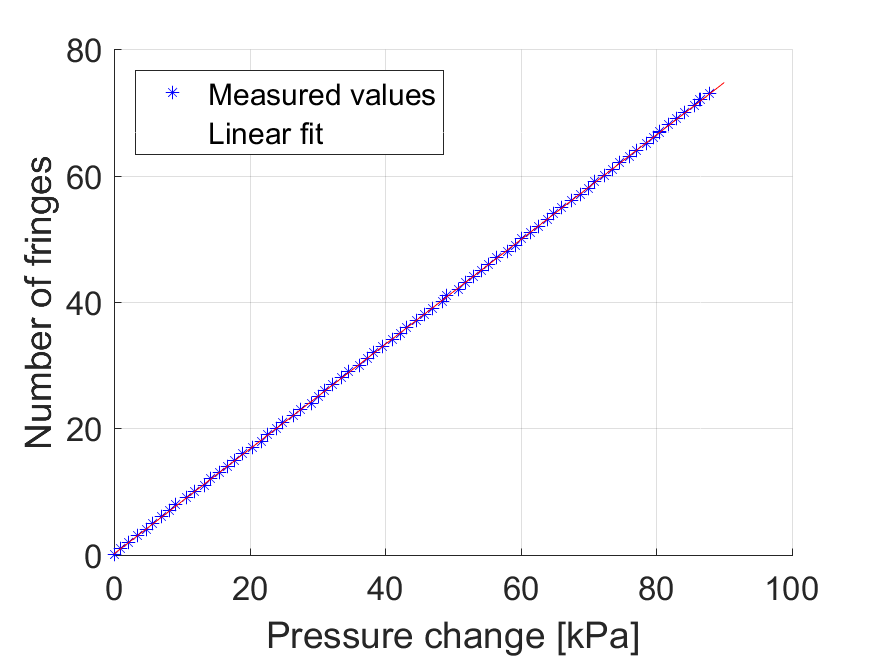
\includegraphics[width=\textwidth]{matlab/Air}
    \caption{Air}
    \label{fig:Air}
  \end{subfigure}
  \begin{subfigure}{0.49\textwidth}
    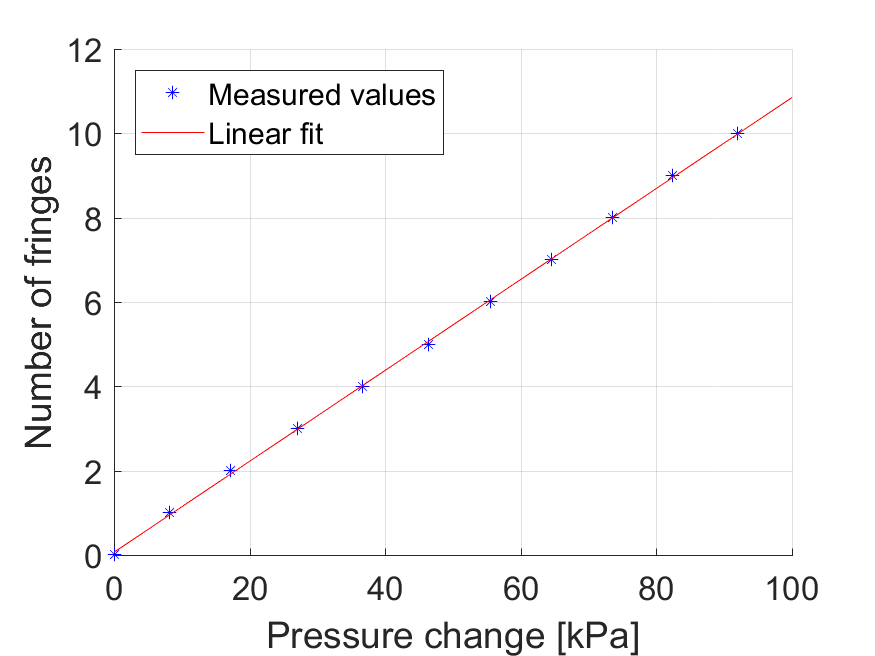
\includegraphics[width=\textwidth]{matlab/Helium}
    \caption{Helium}
    \label{fig:Helium}
  \end{subfigure}
  \begin{subfigure}{0.49\textwidth}
    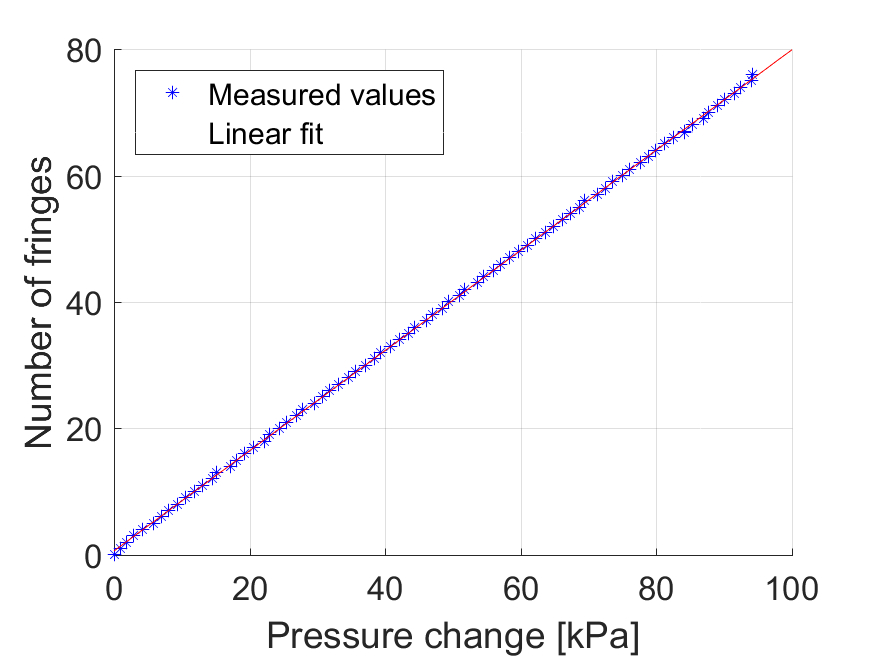
\includegraphics[width=\textwidth]{matlab/Argon}
    \caption{Argon}
    \label{fig:Argon}
  \end{subfigure}
  \begin{subfigure}{0.49\textwidth}
    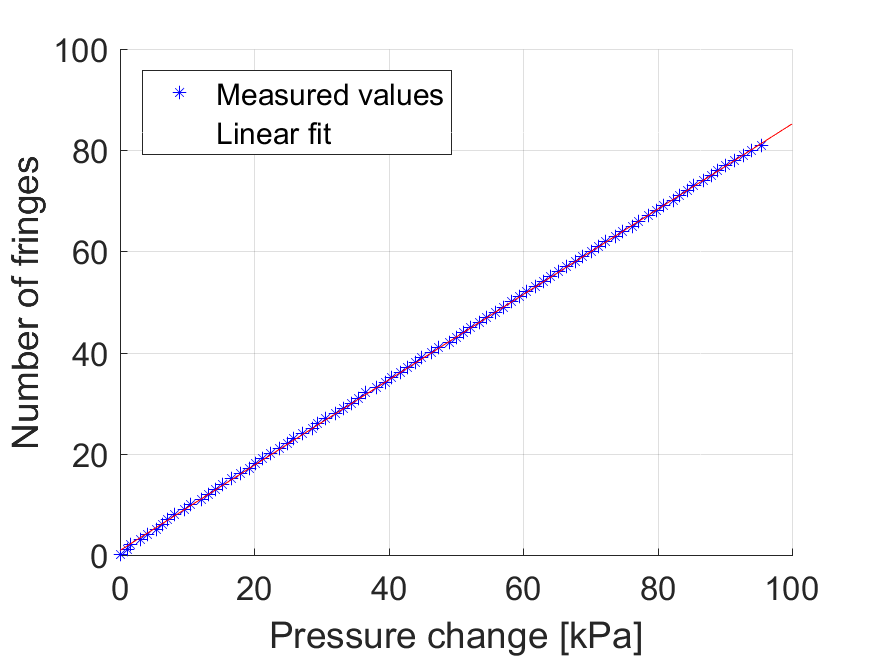
\includegraphics[width=\textwidth]{matlab/Nitrogen}
    \caption{Nitrogen}
    \label{fig:Nitrogen}
  \end{subfigure}
  \caption{Number of fringes and pressure change for the different gases with linear fits. Fitting parameters are found in Tab. \ref{tab:linearFits}}
  \label{fig:measurements}
\end{figure}

\begin{table}[H]
  \centering
  \caption{Fitting parameters for the measured values in Fig. \ref{fig:measurements}. Linear fit on the form $y=\alpha x + \beta$.}
  \label{tab:linearFits}
  \begin{tabular}{l|l|l}
           & $\alpha$ [kPa$^{-1}$]& $\beta$ \\ \hline
  Air      & $0.83(2)$  & $0.16(6)$ \\
  Helium   & $0.11(1)$ & $0.06(5)$ \\
  Argon    & $0.79(3)$ & $0.61(5)$ \\
  Nitrogen & $0.84(2)$ & $0.86(5)$
  \end{tabular}
\end{table}

\begin{table}[H]
  \centering
  \caption{Estimated refractive indexes for the gases including tabulated values \cite{idxAir}-\cite{idxNit}}
  \label{tab:refrIndex}
  \begin{tabular}{l|l|l}%|l}
          & Calculated & Tabulated  \\ \hline %& Error \\ \hline
    Air      & $1.000264(6)$  & $1.000271$  \\ %& $7.05654305 \cdot 10^{-6}$ \\
    Helium   & $1.000034(4)$  & $1.000032$  \\ %& $2.07707264 \cdot 10^{-6}$ \\
    Argon    & $1.000253(9)$  & $1.000261$  \\ %& $8.23800429 \cdot 10^{-6}$ \\
    Nitrogen & $1.000269(6)$  & $1.000276$  \\ %& $7.55338923 \cdot 10^{-6}$
  \end{tabular}
\end{table}

As seen in table \ref{tab:refrIndex} the tabulated values fo the refractive indexes are inside the error margin for helium and argon and slightly outside for air and nitrogen. Notice that the relative error is wastly larger for helium than for the others since it generated fewer fringers due to its smaller index of refractive. Note also that the calculated values are lower compared to the tabulated values for all gases but helium indicating that there might be a systematic error that is unknown. One reason for this could be that the measurements was not taken from perfect vaccum. The pump that was used to generate vaccum only achieved about 0.2-0.4kPa of pressure which intruduces a shift of the measurements. Since the refractive index at this pressure is still approximatly one in Eq. \ref{eq:refrInd}, only the right hand side would shift which would introduce a slightly higher slope $\alpha$. Then question then would be why the refracted index of helium was higher. This could be due to that the lack of measurements overtake this error in the opposite direction.

Another hypothesis of the systematic error is that the gas chamber contained a mix of different gases, most probably air since the pump device was unplugged between measuring the different gases. If the chamber had a combination of air and the other gas examined, it would result in a index of refraction slightly tilted towards the value for air. This theory would overestimate all index of refractions which are lower compared to air, as well as underestimating the ones with higher index of refraction. For our measuremnts this theory holds for helium and nitrogen. But does not explain the error relating to air index of refraction. The most trivial explination would be that we have underestimating the errors in the equipment used, which would make our estimated/calculated errors smaller than the true errors.


%All the tabulated values for index of refraction is within the calculated ones error of margin, as seen in Tab. \ref{tab:refrIndex}. The major thing to notice from the results is that the error margin for helium is approximatly five times larger than the errors for the other gases. This is expected, since helium generated only $10$ fringes while the other gases generated about $70-80$ fringes (i.e. alot more).
